\documentclass[a4paper,12pt]{article}

%%% Работа с русским языком
\usepackage{cmap}					% поиск в PDF
\usepackage{mathtext} 				% русские буквы в формулах
\usepackage[T2A]{fontenc}			% кодировка
\usepackage[utf8]{inputenc}			% кодировка исходного текста
\usepackage[english,russian]{babel}	% локализация и переносы

%%% Дополнительная работа с математикой
\usepackage{amsfonts,amssymb,amsthm,mathtools} % AMS
\usepackage{amsmath}
\usepackage{icomma} % "Умная" запятая: $0,2$ --- число, $0, 2$ --- перечисление
\usepackage{varwidth,gensymb}
\usepackage{esvect} %вектор
\usepackage{gensymb}
\usepackage{hyperref} %гиперссылки

%% Номера формул
%\mathtoolsset{showonlyrefs=true} % Показывать номера только у тех формул, на которые есть \eqref{} в тексте.

%% Шрифты
\usepackage{euscript}	 % Шрифт Евклид
\usepackage{mathrsfs} % Красивый матшрифт
\usepackage{indentfirst} % Красная строка после заголовка

%% Свои команды
\DeclareMathOperator{\sgn}{\mathop{sgn}}

%% Перенос знаков в формулах (по Львовскому)
\newcommand*{\hm}[1]{#1\nobreak\discretionary{}
{\hbox{$\mathsurround=0pt #1$}}{}}

%%% Работа с картинками
\usepackage{graphicx}  % Для вставки рисунков
\graphicspath{{images/}{images2/}}  % папки с картинками
\setlength\fboxsep{3pt} % Отступ рамки \fbox{} от рисунка
\setlength\fboxrule{1pt} % Толщина линий рамки \fbox{}
\usepackage{wrapfig} % Обтекание рисунков и таблиц текстом
\usepackage{caption}

%%% Работа с таблицами
\usepackage{array,tabularx,tabulary,booktabs} % Дополнительная работа с таблицами
\usepackage{longtable}  % Длинные таблицы
\usepackage{multirow} % Слияние строк в таблице
\usepackage{multicol}
% в преамбуле
\usepackage[left=2cm,right=2cm,
top=2cm,bottom=2cm,bindingoffset=0cm]{geometry}

%%% Заголовок


\date{\today}

\begin{document} % конец преамбулы, начало документа
\begin{titlepage}
\
\vspace{20em}

\begin{center}
\Large Фазовые переходы 2-го рода
\end{center}

\vspace{22em}

\begin{flushright}
Студентка 1-го курса \\


\end{flushright}

\vspace{\fill}

\begin{center}
Долгопрудный, 2019
\end{center}
\end{titlepage}
\newpage
\tableofcontents 
\newpage

\section{Введение}
Фазой называется термодинамически равновесное состояние вещества, отличающееся от других возможных равновесных состояний того же вещества. 
Переход вещества от одной фазы в другую – фазовый переход – всегда связан с качественными изменениями свойств вещества и сопровождается скачкообразными изменениями каких-то величин, характеризующих свойства вещества. Тем не менее остается непрерывным удельный термодинамический потенциал $\varphi(T, P)$ 

Различают фазовые переходы двух типов. Фазовые превращения, при которых первые производные термодинамического потенциала меняются скачком, называются фазовыми переходами первого рода. Фазовые превращения, при которых первые производные остаются непрерывными, а вторые - меняются скачком, называются фазовыми переходами второго рода.\\


\section{Фазовые переходы первого рода}
Рассмотрим фазовые переходы первого рода. Так как они характеризуются скачкообразным изменением одной или нескольких величин:
\[s = -\left(\frac{\partial \varphi}{\partial T}\right)_P, \ \ \ \upsilon = -\left(\frac{\partial \varphi}{\partial P}\right)_T\]
Скачкообразное изменение удельной энтропии означает, что фазовое превращение происходит с выделением или поглощением тепла: $q = T(s_2 - s_1)$ - теплота фазового перехода отлична от нуля.\\

\section{Изменения величин при фазовых переходах второго рода}
При фазовом превращении второго рода удельная энтропия и объем остаются непрерывными. Это значит, что переход происходит без выделения или поглощения тепла, но скачкообразно меняются вторые производные $\varphi$:
$$ c_p = T\left(\frac{\partial s}{\partial T}\right)_P = -T\left( \frac{\partial^2 \varphi}{\partial T^2}\right)_P$$
$$\alpha = \frac{1}{\upsilon}\left(\frac{\partial \upsilon}{\partial T}\right)_P = \frac{1}{\upsilon} \frac{\partial^2 \varphi}{\partial P \partial T}$$
$$\gamma = - \frac{1}{\upsilon}\left(\frac{\partial \upsilon}{\partial P}\right)_T = \left(\frac{\partial^2 \varphi}{\partial P^2}\right)_T$$
Тут мы использовали соотношение $\varphi(T,P) = -sdT + \upsilon dP$, из которого следуют выражения для частных производных $\varphi$.

Таким образом, при фазовых превращениях второго рода происходит скачкообразное изменение таких величин: \\
$\cdot$ удельная теплоемкость $c_P$\\
$\cdot$ температурный коэффициент объемного расширения $\alpha = \frac{1}{\upsilon_0}\left(\frac{\partial \upsilon}{\partial T}\right)_P$\\
$\cdot$ изотермический коэффициент сжатия вещества $\gamma = - \frac{1}{\upsilon}\left(\frac{\partial \upsilon}{\partial P}\right)_T$ \\

Рассмотрим ещё одну отличительную черту фазовых переходов второго рода. Как мы знаем, при фазовом превращении первого рода сначала образуются зародыши новой фазы, которые растут, заполняя весь объем. При фазовом переходе второго рода превращение происходит сразу во всем объеме в результате непрерывного изменения кристаллической решетки, т.е. взаимного расположения частиц в решетке. Таким образом, может измениться симметрия решётки. Например, решетка с низкой симметрией может перейти в решётку с более высокой симметрией.	\\

\section{Механизм фазового перехода}
Основную роль в фазовых превращениях играют флуктуации физических величин. Вдали от точки фазового перехода они(флуктуации энергии, плотности и других связанных с ними физических величин) возникают в малых объемах и сразу же рассасываются, но если температура и давление в веществе близки с критическим, то в объеме флуктуаций становится возможным возникновение новой фазы, которая будет являться зародышем, и в последствии увеличиваться. Это является одной из причин сложности создания метастабильных состояний. Например, переохлажденная чистая вода может существовать при температуре $-10\degree C$ длительное время, но на более низких температурах возникающие флуктуации будут слишком высоки, и такие состояния оказываются труднодоступными, либо невозможными.\\

При фазовых переходах флуктуации могут развиваться по разному:\\
$\cdot$ При фазовом переходе первого рода флуктуации(энергии и плотности) происходят все чаще при приближении к точке перехода, и несмотря на то, что каждая флуктуация охватывает малый объем, они могут привести к образованию макроскопического зародыша новой фазы.\\
$\cdot$ При фазовом переходе второго рода, как мы отмечали ранее, новая фаза образуется сразу во всем объеме, а значит, микроскопические флуктуации не могут привести к переходу сами по себе. Но их механизм в данном случае устроен по-другому, флуктуации охватывают все большую часть при приближении к критической температуре и происходят во всем объеме, когда достигают её. Когда новая фаза установилась, они начинают затухать и снова становятся микроскопическими и кратковременными.\\

\newpage
\section{Соотношения Эренфеста}
Так как превращения второго рода происходят при непрерывных $s$ и $\upsilon$, то $\frac{s_1 - s_2}{\upsilon_1 - \upsilon_2}$ вообще говоря не определено, а значит уравнение Клапейрона-Клаузиуса:
\[\frac{dP}{dT} = \frac{q}{T(\upsilon_1 - \upsilon_2)},\]
где $q = T(s_1 - s_2)$, которым можно пользоваться при рассмотрении фазовых превращений первого рода, теряет смысл.

Соотношениями Эренфеста называются следствия непрерывности $s$ и $\upsilon$ при фазовых переходах второго рода. Рассмотрим $s = s(T,P)$:
\[ds = \left(\frac{\partial s}{\partial T}\right)_P dT + \left(\frac{\partial s}{\partial P}\right)_T dP\]
Воспользовавшись соотношениями из предыдущего пункта, получим
\[ds = \frac{c_P}{T}dT - \left(\frac{\partial \upsilon}{\partial T}\right)_P dP\]
Запишем это выражение для каждой фазы и рассмотрим точки (T,P) и (T + dT, P + dP) на кривой фазового равновесия:
\[ds_1 = \frac{c_{1P}}{T}dT - \left(\frac{\partial \upsilon_1}{\partial T}\right)_P dP,\;ds_2 = \frac{c_{2P}}{T}dT - \left(\frac{\partial \upsilon_2}{\partial T}\right)_P dP\]
Из непрерывности удельной энтропии $ds_1 = ds_2$:
\[(c_{2P} - c_{1P})\frac{dT}{T} = \left( \left(\frac{\partial \upsilon_2}{\partial T}\right)_P - \left(\frac{\partial \upsilon_1}{\partial T}\right)_P \right) dP\]
Обозначив $\Delta c = c_{2P} - c_{1P}$ и $\Delta \left( \frac{\partial \upsilon}{\partial T} \right)_P = \left(\frac{\partial \upsilon_2}{\partial T}\right)_P - \left(\frac{\partial \upsilon_1}{\partial T}\right)_P$ получим другую форму записи
\[\Delta c_P = T \Delta \left( \frac{\partial \upsilon}{\partial T} \right)_P \frac{dP}{dT}\]
Это соотношение называется первым соотношением Эренфеста.

Рассмотрев $s = s(T,\upsilon)$, аналогичным образом получим второе соотношение Эренфеста:
\[\Delta c_{\upsilon} = -T \Delta \left( \frac{\partial P}{\partial T} \right)_{\upsilon} \frac{d\upsilon}{dT}\]

Из рассмотрения $s = s(\upsilon, P)$
\[\Delta \left( \frac{\partial \upsilon}{\partial T} \right)_P = \Delta \left( \frac{\partial P}{\partial T} \right)_{\upsilon} \frac{d\upsilon}{dP}\]

Наконец, рассмотрев $\upsilon = \upsilon(T,P)$, из непрерывности $\upsilon$:
\[\Delta \left( \frac{\partial \upsilon}{\partial T} \right)_P = - \Delta \left( \frac{\partial \upsilon}{\partial P} \right)_T \frac{dP}{dT}\]

Следует заметить, что соотношения Эренфеста имеют ограниченую область применимости. Не всегда вторые производные термодинамического потенциала в точках фазовых превращений остаются конечными. Например, при переходе вещества из ферромагнитного в парамагнитное состояние $c_P$ стремится к бесконечности, когда температура стремится к температуре перехода. А это означает стремление к бесконечности также производной $\left({{{\partial s} \over {\partial T}}}\right)_{P}$, а с ней и производной $\left({{{\partial ^{2}\varphi } \over {\partial T^{2}}}}\right)_{P}.$\\


\section{Пример. Переход He I $\rightarrow$ He II}
Рассмотрим один из примеров фазовых переходов второго рода: превращение гелия из обыкновенного жидкого состояния(гелий I) в его жидкую модификацию(гелий II). Характерная особенность фазовой диаграммы гелия - отсутствие кривой возгонки. Это значит, что ни при каких условиях твердый гелий не может быть в равновесии со своим паром. При охлаждении жидкого гелия при определенной температуре(зависящей от внешнего давления), называемой $\lambda$-точкой он испытывает фазовый переход второго рода и переходит в гелий II(при давлении < ~25 атм.). Эта модификация продолжает оставаться жидкой до абсолютного нуля . Все прочие вещества при абсолютном нуле могут находится в твердом состоянии. 

Жидкий гелий II обладает удивильтельным свойством сверхтекучести(нулевая вязкость), открытым П.Л.Капицей.

Отметим, что понижая температуру, гелий невозможно перевести в твердое состояние при атмосферном давлении, для этого требуются давления выше 25 атм, причем оно зависит от температуры. При 50К гелий твердеет при 7000 атм.

Объяснение многих свойств гелия вытекают из квантовой физики. Согласно квантовой теории частицы при абсолютном нуле обладают энергией(называемой нулевой энергией), тем больше, чем меньше масса атомов. Так, атомы гелия обладают наибольшей, после водорода, нулевой энергией. С другой стороны, благодаря особенностям строения атома гелия силы взаимодействия между ними очень малы.  Таким образом, при малых силах взаимодействия нулевая энергия оказывается достаточной для того, чтобы препятствовать атомам гелия образовать кристаллическую решетку. Только с помощью колоссального давления это становится возможным.
Таким образом, при низких температурах именно нулевая энергия, а не энергия теплового движения, определяет поведение.
Водород не обладает такими свойствами, хотя его нулевая энергия ещё больше, потому что энергия взаимодействия между атомами водорода много больше, чем у гелия: в твердом водороде нулевая энергия составляет половину полной энергии, а в гелии ~80$\%$. В лёгком изотопе гелия $He^{3}$ нулевая энергия составляет $~95\%$ полной энергии.

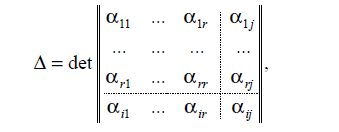
\includegraphics[scale=0.5]{pic1.png}

Другие примеры: переходы металлов (Fe, Cot Ni) из парамагнитного
состояния в ферромагнитное, переходы параэлектрик-сегнетоэлектрик, переходы металлов из обычного состояния в сверхпроводящее.

\newpage
\section{Заключение}
Фазовые переходы второго рода - очень сложное и интересное явление. Процессы, происходящие в непосредственной близости точки перехода, ещё не исследованы до конца, и полная картина поведения физических величин в условиях больших флуктуаций ещё только создается. Также эксперементально не подтверждено существование фазовых переходов третьего рода. Вещества, претерпевшие фазовый переход второго рода, обладают уникальными свойствами, такими как сверхтекучесть и сверпроводимость, которые активно используются в промышленности.


 
% даём указание на включение данного место в оглавление как секции (\section)
\addcontentsline{toc}{section}{Список литературы}
 
%далее сам список используевой литературы
\begin{thebibliography}{}
    \bibitem{litlink1}  Кикоин А.К., Кикоин И.К. Общий курс физики. Молекулярная физика. Издание второе, переработанное - М.: 1976. - 480 с.
    \bibitem{litlink2}  Сивухин Д. В. Общий курс физики: Учеб. пособие для вузов В 5 т. Т. 2. Термодинамика и молекулярная физика — 6-е изд., стереот. —
М.: ФИЗМАТЛИТ, 2016. — 544 с.
	\bibitem{litlink3} Гуфан Ю.М. Структурные фазовые переходы. М.:
Наука, 1982. 302 с.
\end{thebibliography}

\end{document}	